\chapter{Fixing ADD\_ADDR}
\label{chap:addaddr2}

\section{The ADD\_ADDR2 format}
There is an ongoing effort to move the current MPTCP specification \ref{6824} from Experimental to Standard Track. Solving the ADD\_ADDR vulnerability is believed to be a fundamental step to reach the required security standards for the transition to happen.
By analyzing the nature of the vulnerability, various proposals have been elaborated to modify the design of the ADD\_ADDR option [\rfc{7430}]. The conceptual flaw behind the option is that no secret material related to the ongoing MPTCP is included. The only security mechanism connected to such message is indeed the TCP-level sequence and acknowledge numbers, that an attacker has to know in order to inject such message into an ongoing session.
A possible solution could be to add the receiver token of the connection as a field in the ADD\_ADDR option. Such token, exchanged only during connection establishment via the MP\_CAPABLE option, is supposed to be unknown to the attacker that in turns would not be able to forge a valid ADD\_ADDR message. This solution wouldn't be effective if the attacker is able to eavesdrop the keys during the initial handshake; keys' eavesdrop is indeed a security concern related to MPTCP [ref to section on Keys' Eavesdrop], and for this reason it is not advisable to add such information in clear inside the ADD\_ADDR option, since that would give more opportunities for eavesdropping.
Another possibility would be to maintain the ADD\_ADDR format unchanged but to block the attack at a later stage. For example, if the destination address of the SYN packet is added as part of the message used to calculate the HMAC value, the attacker wouldn't be able to recompute the HMAC value after modifying the destination address. However, since addresses are not a stable piece of information in a network with NATs, using the destination address to calculate the HMAC might not work.
In order to achieve higher security levels maintaining NAT compatibility, a third option has been proposed with positive feedback. The idea is to add to the ADD\_ADDR option a new field containing the truncated HMAC value (rightmost 64 bits) calculated as follow: the \textit{key} is the MPTCP key of the sender as originally agreed in the MP\_CAPABLE handshake; the \textit{message} is the concatenation of the previous three fields in packet: Address ID, advertised IP address, and Port. The new format (figure \ref{fig:addaddr2}) has been formally specified for the first time in \rfc{6824bis-04}, but a slight modification will be introduced in \rfc{6824bis-05}, as explained in the following sections.

\begin{figure}[!htb]
\centering
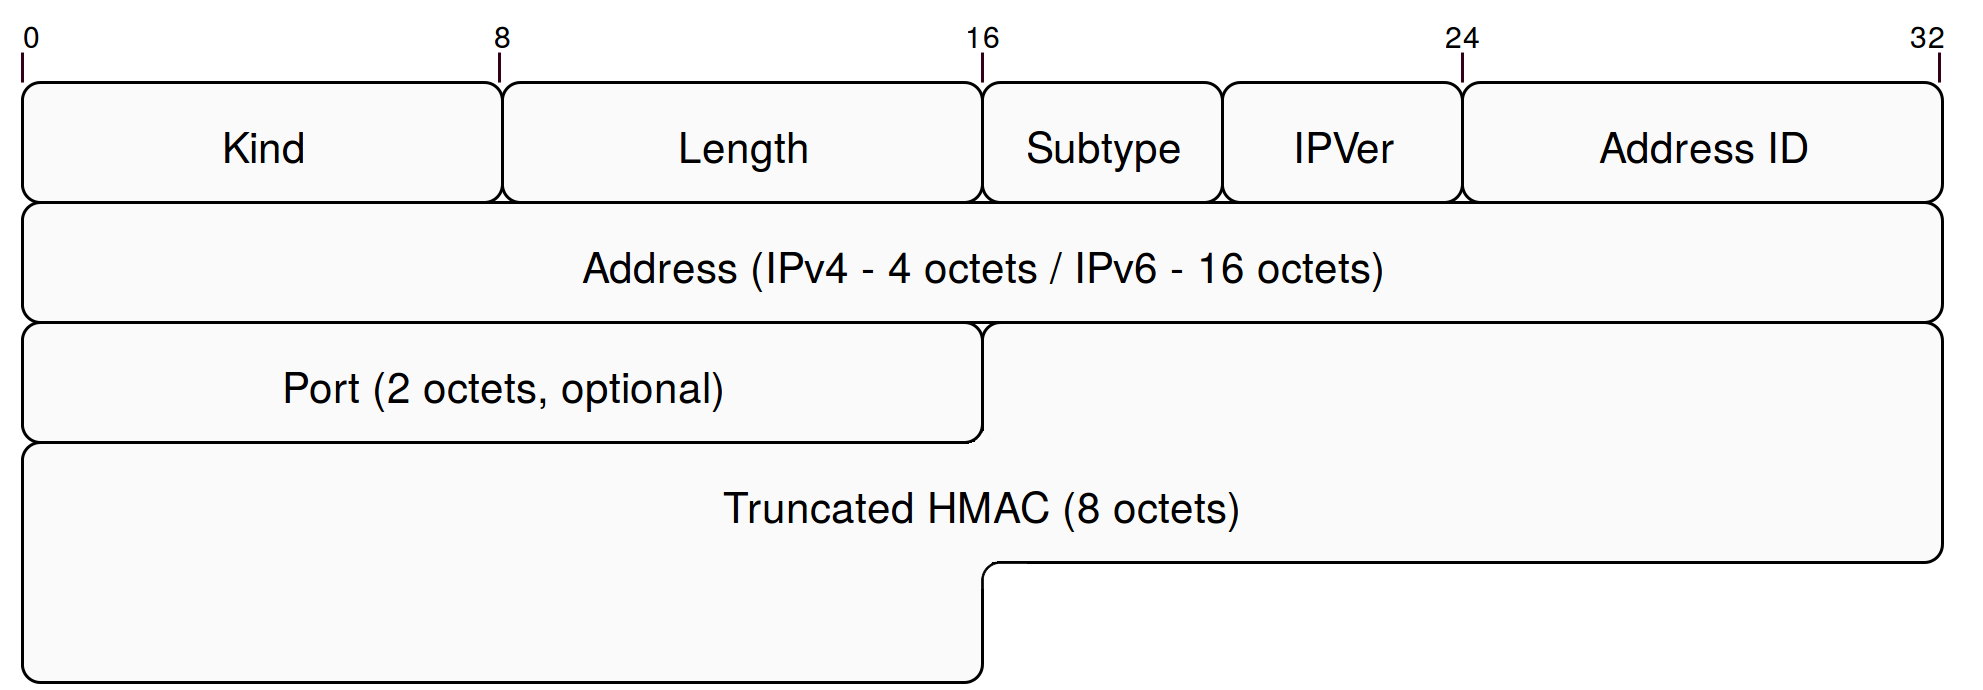
\includegraphics[width=0.75\textwidth]{images/addaddr2}
\caption{ADD\_ADDR2 option}
\label{fig:addaddr2}
\end{figure}

Such format would require the attacker to know the key in order to forge a valid ADD\_ADDR2 message, but such key is not exposed as in the case of the previous solution. Albeit, if the attacker is able to eavesdrop the keys during connection initiation it would be possible to exploit the same vulnerability even with the new address format. More experiments about this case are reported in section [ref to the experimental evaluation section]. Possible mitigations for such threat are explained in section [ref to keys' eavesdrop section 3.3.2].

The keys' eavesdrop threat is a partial-time on-path eavesdrop, a category that is considered less critical in terms of security concerns. Such keys' eavesdrop procedure in MPTCP has an almost identical counterpart in SCTP, when the SCTP-AUTH extension is used without pre-shared keys [\rfc{5061}]. In these regards the same security levels of SCTP would be reached in MPTCP by upgrading ADD\_ADDR to ADD\_ADDR2. Since SCTP is Standard Track, ADD\_ADDR2 is indeed considered a sufficient modification of the MPTCP first design to reach the security levels required for the transition to Standard Track.

\section{Implementing ADD\_ADDR2}
The current MPTCP patch added to the TCP stack in the Linux kernel currently counts around 12000 lines of code [\href{http://multipath-tcp.org/mptcp_stats/index.html}{href}]. It is considered the reference implementation for MPTCP and it closely follows RFC standards and set of features. Moreover, a lot of effort has been put into the implementation design in order to make the new protocol acceptable for upstream to the official Linux kernel. For such purpose, it is of paramount importance to keep the added complexity into the TCP stack as low as possible, in order not to jeopardize performance and stability of regular TCP. Nevertheless, high performance is expected for MPTCP. The main architectural concepts related to the control plane of the protocol are now explained, before introducing the modifications related to the new ADD\_ADDR2 format as defined in \rfc{6824bis-04}. 

\subsection{MPTCP in Linux}
With MPTCP in the Linux kernel, three main layers are introduced to guarantee multipath management and retro-compatibility with regular TCP [\href{http://inl.info.ucl.ac.be/publications/multipath-tcp-theory-practice}{href}]. The first element is the \textit{master subsocket}, which provides the interface used by the applications to communicate with the TCP stack. The structure of the master subsocket follows the regular TCP standards, in order to maintain retro-compatibility towards the application layer: in fact this is the only element used by the kernel in case of regular TCP connectivity. The second element is called \textit{multi-path control block (mpcb)} and it is the main brain of MPTCP, handling MPTCP-specific functionalities: the mpcb runs the algorithms that determine when to start or stop subflows, which subflow to chose in order to send a particular piece of data over the network and how to reconstruct the original data from the scattered segments coming from different subflows at the receiver. all the reordering algorithms in the mpcb work at the data-level, while the reordering of the data at the single subflows is handled by the underlying regular TCP. The final element of the MPTCP architecture is the set of \textit{slave subsockets}, the actual endpoints for the multiple MPTCP subflows. Such elements are not visible by the application, but they are handled by the mpcb. 
The master subsocket and the slave subsockets form the pool of subflows used in MPTCP.

% Change "multipath control block" with "meta-socket". mpcb is just a component of the meta-socket
\begin{figure}[!htb]
\centering
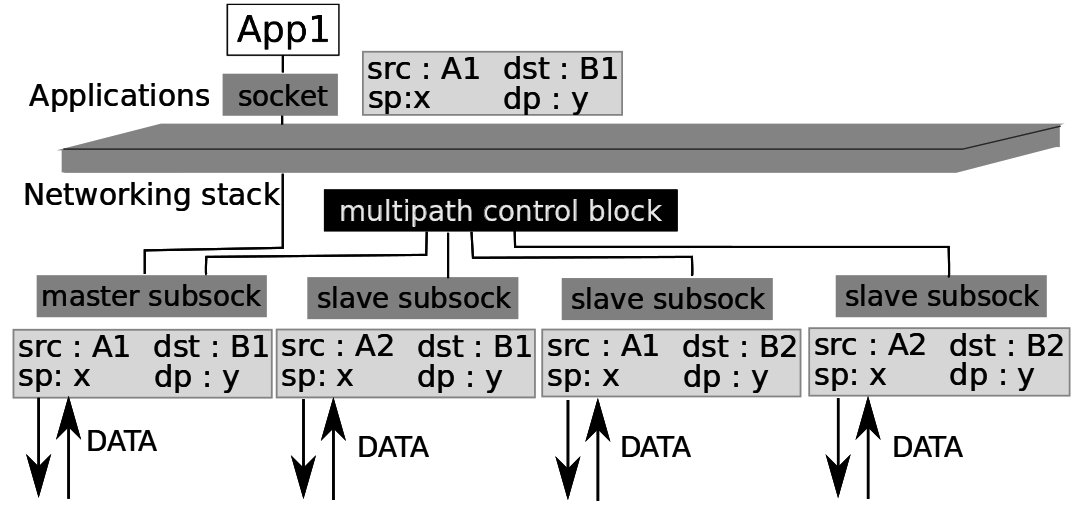
\includegraphics[width=0.75\textwidth]{images/architecture}
\caption{MPTCP Linux architecture}
\label{fig:architecture}
\end{figure}


Analyzing to the actual code implementation related to such architecture, it is mainly composed of several structures linked by pointers. In order to maintain the design-goal if minimizing the impact over regular TCP, when a TCP structure would need additional elements to handle MPTCP-related functionalities, the common choice is to define a new MPTCP-specific structure to store those elements. In this way, upon regular TCP operations, there would be no increase in memory-footprint and all the standard TCP structures would be in place. On top of that, having specific structures for MPTCP code makes it easier to read and understand the MPTCP parts inserted into the TCP stack. For example, a fundamental structure in TCP is the \textit{tcp\_sock} structure, that is used to store the state of a single TCP connection. In MPTCP, additional information for each TCP subflow is needed (for example the Address ID associated to each subflow). A new \textit{mptcp\_tcp\_sock} struct has been defined and each subflow contains a pointer to such new structure.
Also the previously mentioned main architectural element that is the multi-path control block is implemented in code using a new structure called \textit{mptcp\_cb}.

\begin{figure}[!htb]
\centering
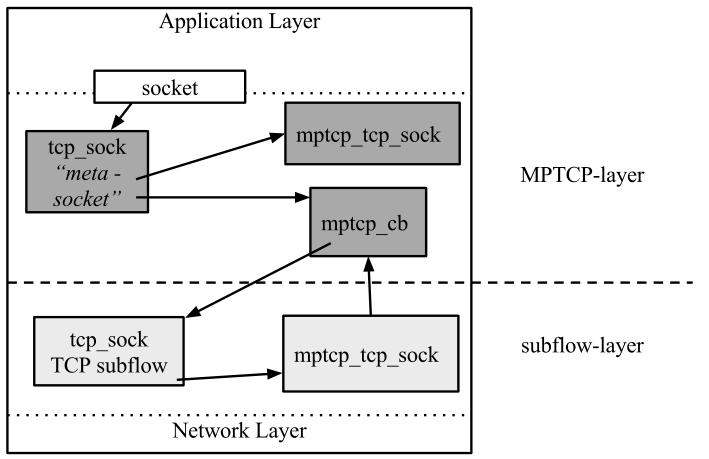
\includegraphics[width=0.7\textwidth]{images/structs}
\caption{MPTCP high-level data structures with relative references}
\label{fig:structs}
\end{figure}
%from Improving MPTCP

The allocation policy for all the new MPTCP structures is lazy-allocation, meaning that MPTCP structures are allocated only if it is detected that both hosts support the new protocol. This choice is again related to the main purpose of not affecting regular TCP when MPTCP fails during negotiation (or later on during the connection lifetime). A downside of this approach is related to the fact that the TCP stack operations are often executed in a soft-interrupt context, that does not allow functions to sleep in order to wait for available memory: this means that memory allocations might fail, forcing a fallback to regular TCP.
Nevertheless, connection setup in an MPTCP-compatible environment requires the client to send a first MP\_CAPABLE segment: this means that, even if no data structure is allocated during this first stage, the client has to generate a random key, and the related token is also calculated to check that it is not already used to identify another MPTCP connection. A reference to the originated \textit{tcp\_sock} structure is saved inside the hashtable used to keep track of the ongoing MPTCP connections. At this point, such \textit{tcp\_sock} is called "meta-socket". After that, if the SYN/ACK from the server does not contain a valid MP\_CAPABLE option, then the client simply removes the reference to the meta-socket from the hashtable before proceeding with a regular TCP handshake procedure. If the server side is MPTCP-compatible and the MP\_CAPABLE is indeed present in the incoming TCP segment, then the MPTCP structures are allocated: \textit{mptcp\_cb} and \textit{mptcp\_tcp\_sock}.
At the server, the status of the connection is not fully operational until the final ACK from the client as required by the TCP three-way handshake. When the SYN packet with MP\_CAPABLE option is processed, a \textit{request\_sock} data structure is allocated that has some additional space for MPTCP-related information with respect to the same structure used for regular TCP option. In case no MP\_CAPABLE option is present in the received SYN packet, the regular TCP version of the \textit{request\_sock} data structure is used, following the same design principles previously explained. The random key and uniqueness of the token are procedures executed at the server in a similar way with respect to the client. If all the MPTCP initialization procedure proceeds as expected, when the server receives the ACK from the client the master-socket is ready and linked to the \textit{mptcp\_cb}.
With the Linux kernel implementation of MPTCP, only the client is allowed to start the establishment of new subflows. There are two main reasons for this: if both client and server start a subflow at the same time, it can be that multiple path are established between the same pair of IP addresses, which can cause problems in some cases. Moreover, clients are often operating behind a NAT, which don't allow server to start new TCP sessions and consequently, they wouldn't allow the server to start a new subflow with the client.

After the connection has been established, multiple subflows can be used with MPTCP and there is a modular path-manager interface to allow flexibility in the heuristic adopted to decide which interfaces can be used and in which manner. In creating a new subflow, the client has to add the MP\_JOIN option inside the SYN packet and, differently from the MP\_CAPABLE scenario, the MPTCP-related structures like \textit{mptcp\_tcp\_sock} are created early on. At this point, failure wouldn't cause fallback to regular TCP and there is no need to risk memory allocation failures upon reception of the SYN/ACK from the server. Even if the subflows in MPTCP resemble regular TCP connections, the initial handshake differs in a way that it now requires four steps to reach fully operational status. The reason for this is that the third ACK now contains the HMAC value calculated by the client that has to be verified and acknowledged by the server before any data can be transmitted on such subflow. 
Regarding the operational flow in the stack upon reception of a SYN packet, there is no early inspection aimed at determining if an MP\_JOIN option is present: that would causes performance degradation in case of regular TCP SYN packets. Instead, the packet is processed with regular TCP stack until, in case of matching with a listening socket, the function \textit{tcp\_v4\_conn\_request()} is called: here the TCP options are scanned, and if MP\_JOIN is present then redirection to MPTCP happens, and the lookup in the hashtable is performed to determine which MPTCP connection the new SYN packet is addressing to. As a new addition required by MPTCP, if there is no matching socket found for the incoming packet, MPTCP still checks if the SYN message contains the MP\_JOIN option via the \textit{mptcp\_lookup\_join()}. At this point, the server creates a request socket that is saved into the hashtable so that it can be retrieved when the client answers with the ACK message during the last stage of the subflow handshake.

This section presented an overview of the most important data structures and functions used in MPTCP to handle connection establishment and subflow management. The following sections will deal with the ADD\_ADDR functionality in the Linux kernel and how this was modified to implement the new format ADD\_ADDR2.

\subsection{Truncated HMAC in ADD\_ADDR}
\label{hmacinaddaddr}
The part of code in the Linux kernel defining the format of every MPTCP options is contained in \textit{include/net/mptcp.h}. For each MPTCP option there is a corresponding structure in this header file that contains all the fields for the option in the right order and with the right format. The ADD\_ADDR option is defined in the \textit{mp\_add\_addr} struct. A first step towards achieving a full implementation of ADD\_ADDR2 is indeed to add the truncated HMAC field to the ADD\_ADDR message and place it after the optional port, both in case of IPv4 and IPv6 (listing \ref{mpaddaddr}, lines 18 and 23).

\begin{lstlisting}[language=c, caption=\textit{mp\_add\_addr struct in the kernel}, label=mpaddaddr]
struct mp_add_addr {
	__u8	kind;
	__u8	len;
#if defined(__LITTLE_ENDIAN_BITFIELD)
	__u8	ipver:4,
		sub:4;
#elif defined(__BIG_ENDIAN_BITFIELD)
	__u8	sub:4,
		ipver:4;
#else
#error	"Adjust your <asm/byteorder.h> defines"
#endif
	__u8	addr_id;
	union {
		struct {
			struct in_addr	addr;
			__be16		port;
			__u8		mac[8];
		} v4;
		struct {
			struct in6_addr	addr;
			__be16		port;
			__u8		mac[8];
		} v6;
	} u;
} __attribute__((__packed__));
\end{lstlisting}

The fields in the data structure indeed resemble the content of ADD\_ADDR as exposed from a high level prospective in section [add section]. 
A \textit{union} is used to define two alternatives for the option's definition, since the advertised IP address can be a longer IPv6 address or a shorter IPv4 address. 
The HMAC value that is computed using the SHA-1 algorithm is of 160 bits, but only its rightmost 64 bits are parsed into the final packet, as can be noticed by the usage of an array of eight elements of kind \_\_u8.  
Particular attention is used to correctly pack the structure, in order to avoid additional padding that could be added by the compiler to align the inner fields for performance reasons. Such padding is unwanted in the final packet sent on wire. The \textit{port} field is optional, meaning that additional care has to be taken when parsing the struct in order to build the packet, as it is explained later in this section.


When the transmission of an ADD\_ADDR2 is triggered, there is a specific function called \textit{full\_mesh\_addr\_signal()} in \textit{net/mptcp/mptcp\_fullmesh.c} that is called to prepare all the fields that will be later on parsed into the outgoing packet. At this point, the fields are saved in a \textit{tcp\_out\_options} structure, defined in \textit{include/linux/tcp.h}. A new \textit{\_\_u64 trunc\_mac} entry has been added to such structure in order to store the new truncated HMAC used in ADD\_ADDR2. 
It is now important to mention that the ADD\_ADDR2 has been designed as a major update for MPTCP, thus being part of the next version bump (MPTCP version 1). Retro-compatibility with version 0 and ADD\_ADDR has to be guaranteed, meaning that the truncated HMAC is added into the ADD\_ADDR message only if version 1 has been established by both hosts during the initial handshake. More about the newly introduced version control is reported in the next section (section [\ref{retrocomp}]).

\begin{lstlisting}[language=c, caption=\textit{New ADD\_ADDR HMAC calculation (outgoing packet)}, label=fullmesh]
 if (mpcb->mptcp_ver >= MPTCP_VERSION_1) {
 u8 mptcp_hash_mac[20];
 u8 no_key[8];

 *(u64 *)no_key = 0;
 mptcp_hmac_sha1((u8 *)&mpcb->mptcp_loc_key,
 		(u8 *)no_key,
		(u32 *)mptcp_hash_mac, 2,
		1, (u8 *)&mptcp_local->locaddr4[ind].loc4_id,
		4, (u8 *)&opts->add_addr4.addr.s_addr);
 opts->add_addr4.trunc_mac = *(u64 *)mptcp_hash_mac;
 }
\end{lstlisting}

In listing \ref{fullmesh} is reported the added code inside \textit{net/mptcp/mptcp\_fullmesh.c} that is used to calculate the HMAC value as previously described. It is possible to notice the "if" statement checking that the MPTCP version in use is indeed 1 or greater. The actual hashing function adopted is \textit{mptcp\_hmac\_sha1}; such function has been also modified to accept as arguments an arbitrary number of messages of arbitrary size (more details about this updated function are reported in section \ref{newhash}). 


Regarding the key used for the HMAC calculation, that is defined as the concatenation of the first two arguments of the hashing function. It corresponds to the key of the sender as defined during the MP\_CAPABLE exchange, followed by 8 bytes initialized to 0 (the \textit{no\_key} field). Even if the 8 trailing bytes are not following the specifications in \rfc{6824bis-04}, these are maintained in order not to change the way the hashing function currently manages the keys for the HMAC computation: \textit{mptcp\_hmac\_sha1} accepts exactly two messages of 8 bytes each and concatenates them to form the final hashing key. This behavior is accepted since it reasonable to assume that in MPTCP the key for any HMAC calculation will always be the concatenation of the two 64-bit keys exchanged via the MP\_CAPABLE option during the initial handshake. This is not the case in the specifications of \rfc{6824bis-04}, but there is no good reason to only use the sender's key at this point. In fact, when an ADD\_ADDR is issued the connection is already up and running, meaning that both hosts know both keys, and concatenating them for the HMAC hashing key improves security overall (an attacker has to know both keys to forge valid HMAC values). These reasonings have been pointed out in the official IETF mailing-list and they have been positively reviewed [\href{https://mailarchive.ietf.org/arch/search/?email_list=multipathtcp&q=RFC6824bis-04+ADD_ADDR2+comments}{href}]: \rfc{6824bis-05}, released in January 2016, modifies the specifications for ADD\_ADDR2 so that both keys are used. For this reason it is acceptable to keep the \textit{no\_key} value in the code as a temporary (incorrect) implementation of \rfc{6824bis-04} standards, since it will be soon replaced with the key of the receiver. 

The HMAC calculation produces 160 bits that are saved in the placeholder called \textit{mptcp\_hash\_mac}, whose pointer is later saved into the previously mentioned new field in \textit{tcp\_out\_options} (line 11 in \ref{fullmesh}).
Later on, in the file \textit{net/mptcp/mptcp\_output.c} the \textit{mp\_add\_addr} is finally constructed by using the elements in the \textit{tcp\_out\_options} data structure, named \textit{opts} in listing \ref{mpoutput}.

\begin{lstlisting}[language=c, caption=\textit{Building ADD\_ADDR2 output message}, label=mpoutput]
 mpadd->kind = TCPOPT_MPTCP;
 if (opts->add_addr_v4) {
 	mpadd->sub = MPTCP_SUB_ADD_ADDR;
 	mpadd->ipver = 4;
 	mpadd->addr_id = opts->add_addr4.addr_id;
 	mpadd->u.v4.addr = opts->add_addr4.addr;
 	if (mpcb->mptcp_ver < MPTCP_VERSION_1) {
 		mpadd->len = MPTCP_SUB_LEN_ADD_ADDR4;
 		ptr += MPTCP_SUB_LEN_ADD_ADDR4_ALIGN >> 2;
 	} else {
 		memcpy((char *)mpadd->u.v4.mac - 2,
 		       (char *)&opts->add_addr4.trunc_mac, 8);
 		mpadd->len = MPTCP_SUB_LEN_ADD_ADDR4_VER1;
 		ptr += MPTCP_SUB_LEN_ADD_ADDR4_ALIGN_VER1 >> 2;
 	}
 }
\end{lstlisting}

The MPTCP version in use is again checked to determine if to add the HMAC field or not. If the version is 1 or greater, then a \textit{memcpy} of the first 8 bytes of the HMAC value is performed to the location \textit{(char *)mpadd->u.v4.mac - 2}; the "-2" is used to start the copying right after the advertised address (IPv4 in this case), thus skipping the optional port field. It is important to mention that the actual implementation of MPTCP for the Linux kernel lacks the feature about port advertisement: more precisely, a port is never added to the ADD\_ADDR option, even if the code to handle a possible port value upon ADD\_ADDR reception is in place and fully operative. Further considerations on port advertisement capabilities can be found in section \ref{portad}. The new ADD\_ADDR2 has different lengths with respect to the previous version, since the 8 bytes truncated HMAC is added. New "len" values are defined, by adding "\_VER1" to the name of the previous definitions: \textit{MPTCP\_SUB\_LEN\_ADD\_ADDR4\_VER1} is 16 (8 in ADD\_ADDR), and \textit{MPTCP\_SUB\_LEN\_ADD\_ADDR6\_VER1} is 28 (20 in ADD\_ADDR). All the code reported so far addresses the IPv4 advertisement, but IPv6 support is provided throughout the entire set of produced patches.


At the receiver side, the ADD\_ADDR2 option is parsed, the HMAC value is calculated (using as HMAC key the MPTCP key of the sender) and a \textit{memcpy} function is used to check that the values coincide. If they do not coincide, the message is simply discarded. Such operations are performed in the function \textit{mptcp\_handle\_add\_addr()} in \textit{net/mptcp/mptcp\_input.c}. Such function is called only if the length of the received option corresponds to the expected values, according to the type of message (ADD\_ADDR or ADD\_ADDR2). This check is performed in another function within the same file, called \textit{mptcp\_parse\_options} (listing \ref{badsize}).

\begin{lstlisting}[language=c, caption=\textit{Check ADD\_ADDR size at the receiver, inside \textit{mptcp\_parse\_option()}}, label=badsize]
	if (!is_valid_addropt_opsize(tp->mpcb->mptcp_ver,
				     mpadd, opsize)) {
 		mptcp_debug("%s: mp_add_addr: bad option size %d\n",
 			    __func__, opsize);
 		break;
\end{lstlisting}

An issue encountered at this point of development was that the function just mentioned was initially called with no reference to the \textit{mpcb} structure where the version of the current MPTCP session is stored. The MPTCP version is no more passed along in the options following the MP\_CAPABLE exchange, meaning that the value can't be retrieved directly from parsing the ADD\_ADDR option. A first workaround was to add the version value in the structure containing the received options, named \textit{mptcp\_options\_received}, before passing the structure to the actual parsing function. Anyway, this might be confusing to the developers, since it looks like the MPTCP version value has been indeed received within the options inside the TCP segment, while it was in reality saved at connection initialization. The final approach to solve the problem involved a slightly more complex changes in the set of function calls related to the parsing of TCP/MPTCP options: as it can be seen in the first line of listing \ref{badsize}, the \textit{tcp\_sock} (\textit{tp}) structure containing the \textit{mpcb} data for the connection is available inside \textit{mptcp\_parse\_option()}, and it can be passed along to the checking function \textit{is\_valid\_addropt\_opsize()}. This required to modify the \textit{tcp\_parse\_options()} function in the TCP stack to pass along the pointer to the \textit{tcp\_sock}, so that it can be retrieved further down within the function calls chain (listing \ref{tcpparse}, last line).

\begin{lstlisting}[language=c, caption=\textit{New definition for \textit{tcp\_parse\_options}}, label=tcpparse]
void tcp_parse_options(const struct sk_buff *skb,
 		       struct tcp_options_received *opt_rx,
 		       struct mptcp_options_received *mopt_rx,
		       int estab, struct tcp_fastopen_cookie *foc);
		       int estab, struct tcp_fastopen_cookie *foc,
		       struct tcp_sock *tp);
\end{lstlisting}

Regarding the \textit{is\_valid\_addropt\_opsize()} function, it has been developed as a separate inline function called inside the "if" statement" for better readability, since the length's check with the additional ADD\_ADDR2 case involves now four possible configurations; the entire function content can be found in the appendix [add appendix reference where the patch is].
Eventually, if the option size is correct and, in case of MPTCP version 1 or higher, the HMAC calculations at the sender and at the receiver match, the advertisement procedure is completed and the receiver can decide if to use the information to open a new subflow.

%Apparently there was a bug there! You can mention it and the related patch. https://listes-2.sipr.ucl.ac.be/sympa/arc/mptcp-dev/2016-02/msg00007.html

\subsection{Retro-compatibility}
\label{retrocomp}
ADD\_ADDR2 is substantial modification of an important design aspect of the MPTCP protocol. ADD\_ADDR2 is indeed non interoperable with the current stable implementation of MPTCP version 0, since the augmented length of the option would cause the older network stack to discard the option right away.
ADD\_ADDR2 is considered part of the new MPTCP protocol version number 1, whose implementation has to guarantee retro-compatibility. For this purpose, a version control mechanism has to be in place so that hosts can agree on the version to use upon initial handshake and successively operate according to such decision. Since ADD\_ADDR2 is the first step towards the implementation of the new features for MPTCP version 1, no version control mechanism was provided at the beginning of the development phase for ADD\_ADDR2. Indeed, version 0 was just an hardcoded value parsed into each MP\_CAPABLE option (option's format is shown in figure \ref{fig:opt_capable}) with no logic attached.


MPTCP version 1 is currently a moving target, so the version bump is not included inside the patch for ADD\_ADDR2 that is just a part of the future changes introduced with the new version (more about this in the section [add ref to "Future Work"]. For this reason, it has been decided to give the system administrator the possibility of dynamically set the MPTCP version via a sysctl call, like the following:

\begin{verbatim}
        sysctl -w net.mptcp.mptcp_version=1
\end{verbatim}

It is possible to identify three main phases in the version agreement procedure, defined in \rfc{6824bis-04}.:

\begin{enumerate}
  \item The client insert the highest available MPTCP version number it supports into the MP\_CAPABLE option;
  \item When the server gets the first MPTCP packet, it checks the version advertised by the client and answer with the highest version it supports that is less or equal to the client's version;
  \item As a last step, the client receives the answer from the server, and it checks that it is indeed a valid version (i.e. it is no greater than the one the client advertised in the first place); at this point, the client can backtrack to regular TCP if it does not wish to use the requested version.
\end{enumerate}

In developing such functionalities, a problem was related to the fact that the user can change the version in use at any time via a sysctl, meaning that it is possible to change the version in the middle of an MPTCP connection. It is not desirable to change such configuration during the MP\_CAPABLE exchange: it is possible that the first MP\_CAPABLE is retransmitted to the passive opener (following standard TCP retransmission procedures), and the version number inside retransmitted packets must not change from the one used in the very first transmission. For this reason, the configured sysctl value is read and initialized for the MPTCP connection at an early stage, namely when \textit{mptcp\_enable\_sock()} in \textit{net/mptcp/mptcp\_ctrl.c} is called; there, the value is saved into the newly introduced field \textit{mptcp\_ver} inside the \textit{tcp\_sock} structure (listing \ref{verphase0}).

\begin{lstlisting}[language=c, caption=\textit{MPTCP version agreement, initializing sysctl value}, label=verphase0]
 void mptcp_enable_sock(struct sock *sk)
 {
 	if (!sock_flag(sk, SOCK_MPTCP)) {
 		sock_set_flag(sk, SOCK_MPTCP);
		tcp_sk(sk)->mptcp_ver = sysctl_mptcp_version;
	...
\end{lstlisting}

Even if the sysctl value is changed by the user after the \textit{mptcp\_enable\_sock()} has been called, the value in \textit{tcp\_sock} for a specific connection is not affected, and that is indeed the value used to create and send the SYN+MP\_CAPABLE option (even in case of retransmissions). 


The same initialization procedure is executed when the MP\_CAPABLE packet is received at the server side, meaning that the code for version agreement at the server also retrieve the local MPTCP version via \textit{tp->mptcp\_ver}, where \textit{tp} is the pointer to the \textit{tcp\_struct} for the connection (listing \ref{verphase2}). The function \textit{mptcp\_reqsk\_new\_mptcp()} in \textit{net/mptcp/mptcp\_ctrl.c} is called and the code in listing \ref{verphase2} is executed to set the highest version available that is not greater than the one advertised by the client. The \textit{mopt} pointer points to the structure containing the received MPTCP options from the client, while \textit{mtreq} is a pointer to the \textit{mptcp\_request\_sock} structure, where the final version chosen by the server is saved for now.

\begin{lstlisting}[language=c, caption=\textit{MPTCP version agreement, phase 2}, label=verphase2]
	if (mopt->mptcp_ver >= tp->mptcp_ver)
		mtreq->mptcp_ver = tp->mptcp_ver;
	else
		mtreq->mptcp_ver = mopt->mptcp_ver;
\end{lstlisting}

The last step of the version agreement involves the final check performed by the client on the version value sent back by the server: it has to be equal or less then the one originally advertised in the first MP\_CAPABLE message. Such check is indeed added to the function \textit{mptcp\_rcv\_synsent\_state\_process()} inside \textit{net/mptcp/mptcp\_input.c} (listing \ref{verphase3}): \textit{tcp\_sk(sk)} is used to obtain the pointer to the \textit{tcp\_sock} structure, where \textit{mptcp\_ver} is retrieved and compared to the server's MPTCP version residing in \textit{mopt->mptcp\_ver}. If the comparison fails, the \textit{fallback} label is hit to trigger the fallback procedure to regular TCP.

\begin{lstlisting}[language=c, caption=\textit{MPTCP version agreement, phase 3}, label=verphase3]
	if (mopt->mptcp_ver > tcp_sk(sk)->mptcp_ver)
		/* TODO Consider adding new MPTCP_INC_STATS entry */
		goto fallback;
\end{lstlisting}

After these messages have been exchanged, if a proper version has been agreed, both hosts will eventually call \textit{mptcp\_create\_master\_sk()} and in turns \textit{mptcp\_alloc\_mpcb()} with the information about the version, so that it is also saved in the MPTCP control block \textit{mptcp\_cb} for the session, from where it will be retrieved to process the ADD\_ADDR option accordingly as explained in section \ref{hmacinaddaddr}.


\subsection{Extending the hashing function}
\label{newhash}
The current implementation of MPTCP in the Linux kernel adopts a specific function for all the HMAC-SHA1 calculations required by the protocol: it is named \textit{mptcp\_hmac\_sha1()} and it is placed inside \textit{net/mptcp/mptcp\_ctrl.c}. Before the introduction of ADD\_ADDR2, only the MP\_JOIN option required such functionality, with a fixed scheme regarding the type and length of the \textit{key} and \textit{message} used as input for the HMAC algorithm: the key is always the concatenation of the two 64-bit MPTCP keys exchanged via the MP\_CAPABLE option, while the message is always the combination or two random nonces of 32 bits each. For this reason, the function has been designed to accept such input values with no flexibility on the length and number of the byte strings passed along for the HMAC computation. The old prototype for \textit{mptcp\_hmac\_sha1()} is shown in listing \ref{oldhmac}.

\begin{lstlisting}[language=c, caption=\textit{Prototype for the old \textit{mptcp\_hmac\_sha1() function}}, label=oldhmac]
void mptcp_hmac_sha1(u8 *key_1, u8 *key_2, u8 *rand_1, u8 *rand_2, 
                     u32 *hash_out);
\end{lstlisting}
 
The old implementation of the function does indeed concatenate the first 8 bytes pointed by \textit{key\_1} and \textit{key\_2} to get the 16 bytes key, and it later concatenates the first 4 bytes of \textit{rand\_1} and \textit{rand\_2} to originate the 8 bytes message. The \textit{hash\_out} pointers references to the placeholder for the final result of the calculation (which is 20 bytes long).


With ADD\_ADDR2 the requirements for the HMAC calculation changed. The hashing key follows the same configuration of the MP\_JOIN case, while the message is now the concatenation of some of the fields in the ADD\_ADDR2 option, namely the single byte Address ID, the advertised address (that can be a 4 bytes IPv4 address or a IPv6 16 bytes address) and, if present, the 2 bytes port value. Instead of implementing a separate hashing function for dealing with this case,  it was decided to extend the current one in order to accept an arbitrary number of message of arbitrary length (checking that the total length doesn't overcome a certain limit). For what concerns the HMAC key, that part is expected not to change for future usage in various parts of MPTCP since it is most likely based on the two MPTCP keys exchanged during the initial handshake. For the message part, the new function uses that C functionality for variable argument lists based on va\_list. The first part of the new hashing function is shown in listing \ref{newhmac}.

\begin{lstlisting}[language=c, caption=\textit{Implementation for the new \textit{mptcp\_hmac\_sha1() function (first part)}}, label=newhmac]
void mptcp_hmac_sha1(u8 *key_1, u8 *key_2, 
                     u32 *hash_out, int arg_num, ...)
{
    u32 workspace[SHA_WORKSPACE_WORDS];
	u8 input[128]; /* 2 512-bit blocks */
	int i;
	int index;
	int length;
	u8 *msg;
	va_list list;

	memset(workspace, 0, sizeof(workspace));

	/* Generate key xored with ipad */
	memset(input, 0x36, 64);
	for (i = 0; i < 8; i++)
		input[i] ^= key_1[i];
	for (i = 0; i < 8; i++)
		input[i + 8] ^= key_2[i];

	va_start(list, arg_num);
	index = 64;
	for (i = 0; i < arg_num; i++) {
		length = va_arg(list, int);
		msg = va_arg(list, u8 *);
		BUG_ON(index + length > 125); /* Message is too long */
		memcpy(&input[index], msg, length);
		index += length;
	}
	va_end(list);

	input[index] = 0x80; /* Padding: First bit after message = 1 */
	memset(&input[index + 1], 0, (126 - index));

	/* Padding: Length of the message = 512 + message length (bits) */
	input[126] = 0x02;
	input[127] = ((index - 64) * 8); /* Message length (bits) */
	...
\end{lstlisting}

In this first section the \textit{input} array is prepared for the subsequent HMAC-SHA1 operations (not reported here). From line 13 to line 16 it is possible to verify that the 16 bytes' key is properly xored with the first 16 bytes of the array as required for the proper HMAC calculation. From line 18 to line 27 the "for" loop scans the function arguments by retrieving two subsequent argument at a time: the first is an integer representing the length of the currently processed message, while the second is the pointer to the actual message. After checking that the total length of the concatenated message is not too long, the message is properly parsed into the \textit{input} array, before advancing the index accordingly and start a new "for" loop. The last part of the code snippet shows some padding additions required by the hashing function. The new API indeed requires to pass along the following set of information, in this order: pointer to the first 8 bytes of the HMAC key, pointer to the following 8 bytes of the key, pointer to the 20-byte placeholder where to save the final result of the HMAC calculation, the number of HMAC message's parts that have to be processed and, finally, the pointers to the various components composing the final HMAC input message, where each pointer has to be preceded by an integer determining the byte-length of the subsequent message. Indeed, this how the function is used to calculate the HMAC value in listing \ref{fullmesh}.


\subsection{Crypto-API in MPTCP}
A major problem was how to deal with the new hashing requirements introduced by ADD\_ADDR2. Extending the current MPTCP hashing function to deal with input messages of arbitrary size is a first point to explain. The second part has to deal with the whole analysis related to adopting the kernel CRYPTO APIs to calculate the HMAC values in MPTCP and why this is not advisable.

\subsection{Port advertisement}
\label{portad}
Port advertisement in ADD\_ADDR is possible according to RFC specifications but it was not part of the implementation at the beginning of the thesis work, so it has been added.

\subsection{IPv6 considerations}
Longer addresses brought some issues related to TCP option fields limitations.


\section{Other contributions}
Another minor part of the thesis work on MPTCP is related to some small contributions to the official RFC documentation and other open-source projects.

\section{Experimental evaluation}
This part should include performance analysis regarding the new format introduced with ADD\_ADDR2. A discussion on how the new format (and all the other modifications introduced with the patches) could impact any aspect of the protocol should be present in this section.
It is possible to add here the other possible solutions for ADD\_ADDR fix, and why they are not good enough. 